%//==============================--@--===========================//%
\clearpage
\subsubsection[5.5.3 Virtual Local Area Network (VLAN)]{$\rightarrow$ Virtual Local Area Network (VLAN)}

\begin{mdframed}
    A \textbf{Virtual Local Area Network (VLAN)} is a network configuration that allows multiple virtual LANs to be defined over a single physical LAN infrastructure. This enables hosts within a VLAN to communicate as if they were exclusively connected to the switch, providing solutions for issues such as lack of traffic isolation, inefficient use of switches, and user management difficulties in modern institutional LANs.
\end{mdframed}

\noindent In port-based VLANs, the switch's ports are divided into groups, with each group forming a VLAN and its own broadcast domain. VLAN switches can be interconnected using two methods: direct connections between VLAN ports or a more scalable approach called \textbf{VLAN trunking}. In trunking, a special port on each switch is configured as a trunk port that belongs to all VLANs. Frames sent to any VLAN are forwarded over the trunk link to the other switch.

\begin{figure}[H]
    \centering
    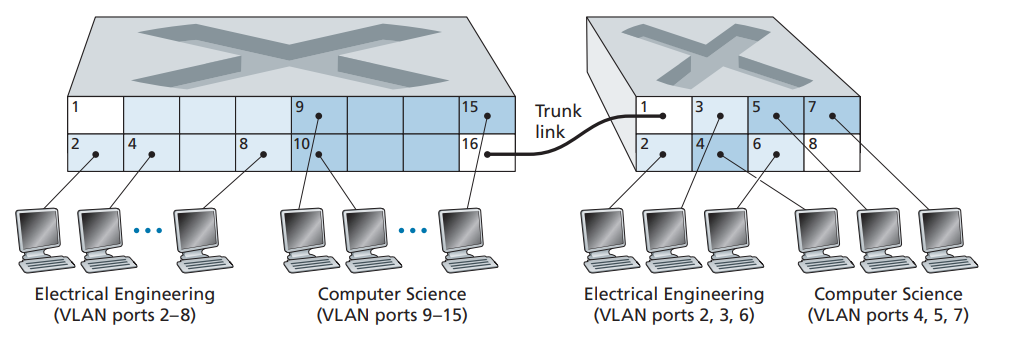
\includegraphics[width = 0.8\linewidth]{img/5/port-based-VLAN.png}
    \caption{Connecting two VLAN switches with two VLANs \cite{Kurose2017}}
    \label{fig:port-based-VLAN}
\end{figure}

\noindent To identify the frame's VLAN membership, the IEEE 802.1Q frame format is used. It extends the standard Ethernet frame by adding a four-byte \textbf{VLAN tag} to the header, containing the \textbf{VLAN identifier} and a priority field. This tag is added and removed by the sending and receiving switches, respectively.

\begin{figure}[H]
    \centering
    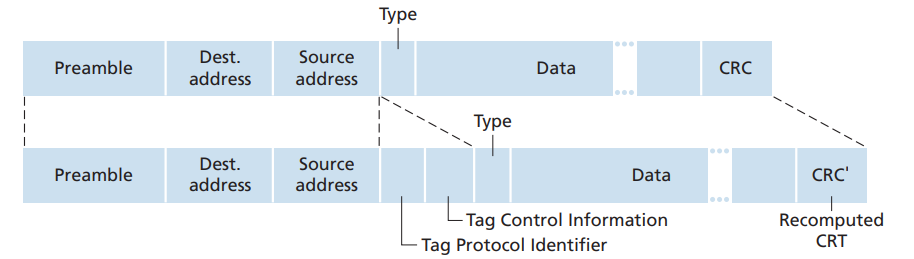
\includegraphics[width = 0.7\linewidth]{img/5/802.1Q-tagged-VLAN-frame.png}
    \caption{Original Ethernet frame (top), 802.1Q-tagged Ethernet VLAN frame (below) \cite{Kurose2017}}
    \label{fig:802.1Q-tagged-VLAN-frame}
\end{figure}

\noindent Besides port-based VLANs, there are MAC-based VLANs where the network manager specifies the set of MAC addresses belonging to each VLAN. VLANs can also be defined based on network-layer protocols and other criteria. It is even possible for VLANs to be extended across IP routers, allowing geographically separated LANs to form a single VLAN.

%//==============================--@--===========================//%
